\documentclass[11pt,a4paper]{report}
\usepackage{amsmath}
\usepackage{amssymb}

\usepackage{graphicx}

\usepackage{listings}
\usepackage{color} %red, green, blue, yellow, cyan, magenta, black, white
\definecolor{mygreen}{RGB}{28,172,0} % color values Red, Green, Blue
\definecolor{mylilas}{RGB}{170,55,241}


\usepackage{graphicx}


\begin{document}
\begin{center}

\LARGE Mek4250 - Mandatory assignment 1
\\
Andreas Thune
\\
\LARGE
16.03.2016

\end{center}
\textbf{Exercise 1}
\\
a) The $H^p$ norm of a function $u(x,y)$ of two variables on $\Omega=(0,1)^2$ is defined as follows: 
\begin{gather}
||u||_{H^p(\Omega)}^2 = \sum_{i=0}^p \sum_{j=0}^{i}\binom {i} {j} ||\frac{\partial^i u}{\partial^j x \partial^{i-j}y}||_{L^2(\Omega)}^2 
\end{gather}
In our case $u(x,y)=sin(k\pi x)cos(l\pi y)$. We easily see that the derivative of this function can be expressed with the following formula: 
\begin{gather}
\frac{\partial^i u(x,y)}{\partial^j x \partial^{i}y} = (k\pi)^j(l\pi)^if_j(k\pi x)g_j(l\pi y)
\end{gather}
were $f_j$ is the j-th derivative of $sin(x)$ and $g_i$ is the i-th derivative of $cos(y)$. Now lets look at the $L^2$ norm of (2).
\begin{gather*}
||\frac{\partial^i u(x,y)}{\partial^j x \partial^{i}y}||_{L^2(\Omega)}^2 = (k\pi)^{2j}(l\pi)^{2i} \int\int_{\Omega} f_j(k\pi x)^2g_i(l\pi y)^2 dxdy \\
= (k\pi)^{2j}(l\pi)^{2i}\int_0^1f_j(k\pi x)^2dx\int_0^1g_i(l\pi y)^2dy
\end{gather*}
Since $f_j^2$ and $g_i^2$ are:
\begin{displaymath}
   f_j(x)^2 = \left\{
     \begin{array}{lr}
       sin^2(x) &  \text{j even} \\
       cos^2(x) &  \text{j odd}
     \end{array}
   \right.
\end{displaymath}
and 
\begin{displaymath}
   g_i(y)^2 = \left\{
     \begin{array}{lr}
       cos^2(y) &  \text{i even} \\
       sin^2(y) &  \text{i odd}
     \end{array}
   \right.
\end{displaymath}
and since $$\int_0^1sin^2(l\pi y)dy=\int_0^1cos^2(l\pi y)dy=\frac{1}{2} $$
we get the following expression for the square of the $L^2$ norm of a general derivative of u:
\begin{gather*}
||\frac{\partial^i u(x,y)}{\partial^j x \partial^{i}y}||_{L^2(\Omega)}^2 = \frac{1}{4}(k\pi)^{2j}(l\pi)^{2i} 
\end{gather*}
If we plug this into (1), we get
\begin{gather*}
||u||_{H^p(\Omega)}^2 = \frac{1}{4}\sum_{i=0}^p \sum_{j=0}^{i}\binom {i} {j}(k\pi)^{2j}(l\pi)^{2(i-j)}  
\end{gather*}
\\
\\
\begin{figure}
  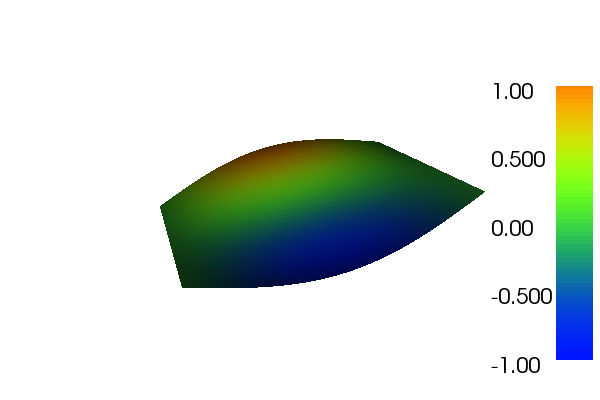
\includegraphics[width=\linewidth]{dolfin_plot_0.png}
  \caption{Plot of numerical solution u for $k=l=1$ and $h=64$. See that everything lies between $-1$ and $1$ as one would expect from a product between sine and cosine functions. Notice also that the solution is smooth}
  \label{Fig 1}
\end{figure}
b) To solve the equation numerically I need to derive the variational form of the equation. Since our boundary conditions are homogeneous Neumann and Dirichlet, I will ignore them completely. Our equation is then:
\begin{align*}
-\bigtriangleup u = f \\
\end{align*} 
Multiply this with testfunction $v$, and integrate over $\Omega=(0,1)^2$:
\begin{align*}
-&\int_{\Omega}\bigtriangleup uvdx=\int_{\Omega}fvdx \\
\iff &\int_{\Omega}\bigtriangledown u\cdot\bigtriangledown vdx = \int_{\Omega}fvdx
\end{align*}
This is our variatonal form, that we write in FEniCS. To get it we use partial integration. We also need to find $f=-\bigtriangleup u$. Since we know $u$ this is simple.
\begin{align*}
f&=-\bigtriangleup u=-\bigtriangleup sin(k\pi x)cos(l\pi y) \\
&= ((k\pi)^2 +(l\pi)^2)sin(k\pi x)cos(l\pi y)
\end{align*} 
\\
\\
In this exercise we were supposed to find the $L^2$ and $H^1$ error when solving our equation numerical for both elements of order 1 and 2, and for different values of $k$ and $l$. To make it short I will only present my results for $k=1$. The code for this exercise is added at the end, and the results are added at the end of the code. What we see from the error, is that it is small for k and l small, but big when k or l get big. This is especially true for the $H^1$ error. The reason for this is that big k and l means that our exact solution will "go up and down" very quickly, and since we are using a quite coarse mesh, we will get aliasing. To illustrate this I have added the plots of our numerical solutions for $k=l=1$ and $k=l=100$ when $\frac{1}{h}=64$ and using $P1$ elements. 
\begin{figure}
  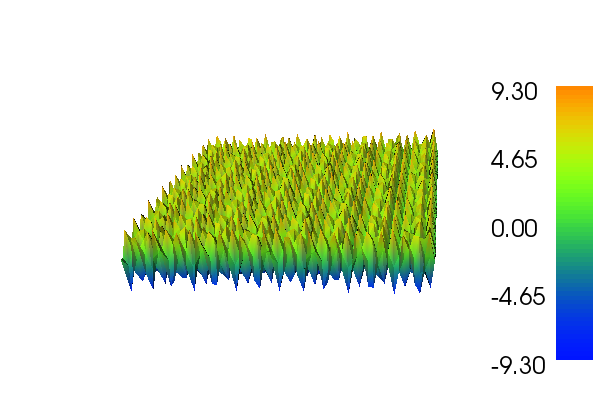
\includegraphics[width=\linewidth]{dolfin_plot_1.png}
  \caption{Plot of numerical solution u for $k=l=100$ and $h=64$. Now the values of u exceed both $-1$ and $1$, and it also does not look smooth. This is due to aliasing. }
  \label{Fig 2}
\end{figure}
\\
\\
c) Since I implemented the norm in a), I have measured the convergence rate using all equations and errors, and also the convergence rate for each problem separately. This means I have tried to fit 
\begin{align}
\frac{||u-u_h||_{H^p}}{||u||_{H^{q+1}}} \ \text{ to } \ Ch^{\alpha} 
\end{align} 
where $u$ is exact solution to the equation for all l and k, and $u_h$ is the same numerically. I also calculated convergence rate while holding k and l fixed, using the following:
\begin{align}
||u-u_h||_{H^p} \ \text{ to } \ Ch^{\alpha} 
\end{align}
Using $P1$ elements I got the following result when estimating convergence for (3):
\begin{center}
    \begin{tabular}{| l | l | l |}
    \hline
     & Convergence rate & Constant  \\ \hline
    $L^2$ &  1.776496& 0.041508 \\ \hline
    $H^1$ &  0.911748 & 0.181145 	\\ \hline
    \end{tabular}
\end{center}
For $P2$ the result was:
\begin{center}
    \begin{tabular}{| l | l | l |}
    \hline
     & Convergence rate & Constant  \\ \hline
    $L^2$ & 2.570886 & 0.000820 \\ \hline
    $H^1$ & 1.491997 &  0.003164	\\ \hline
    \end{tabular}
\end{center}
Theoretically we would expect 
\begin{align*}
\frac{||u-u_h||_p}{||u||_{q+1}}  \leq Ch^{q+1-p}
\end{align*}
In the expression above $q$ represent the order of the element used in our finite element method. We see that our numerical estimates of the convergence rate in all cases are lower than what we would expect. This could indeed be a result of the aliasing we get because of our coarse mesh. As I said I also checked convergence for $(k,l)$ pairs separately, and this is the $L^2$ convergence rates I got for $P1$ elements :
\begin{center}
    \begin{tabular}{| l | l | l | l |}
    \hline
     & $k=1$ & $k=10$ & $k=100$  \\ \hline
    $l=1$ & 1.980241 & 1.665838 &2.253570  \\ \hline
    $l=10$ & 1.663255 &  1.190830 &	1.298707\\ \hline
    $l=100$ & 2.265711 &  1.367577 & 2.302735	\\ \hline
    \end{tabular}
\end{center}
One remark to these numbers, are that even though the convergence rate is good for k and l around $100$, the constant is in these cases really big, and it is therefore simple to get good convergence. The bad convergence occurs around k and l equal to $10$. This is probably because this is a borderline case where our mesh is almost good enough to avoid aliasing. The rest of the results is found in the code.
\\
\\ 
\textbf{Exercise 2}
\\
a) Assume our solution is on the form $u(x,y)=X(x)Y(y)$. If we plug this into our equation and assume that both $X$ and $Y$ are nonzero, we get:
\begin{align*}
&-\mu(X''Y+XY'') + X'Y = 0 \iff \frac{- \mu X''+X'}{X} - \mu\frac{Y''}{Y}=0 \\
&\iff - \mu X''+X'=\lambda X \ \text{and} \ \mu Y'' = \lambda Y
\end{align*} 
Now lets look at the boundary conditions, starting withe the Dirichlet conditions:
\begin{align*}
u(0,y)=0 \iff X(0)Y(y)=0 \Rightarrow X(0)=0 
\end{align*}
Since $Y(y)=0$ would be a contradiction.
\begin{align*}
u(1,y)=1 \iff X(1)Y(y)=1 \Rightarrow Y(y)=1/X(1)
\end{align*} 
This means that $Y(y)$ is a constant. This does not contradict our Neumann boundary conditions, since they say that the y-derivative is zero at $y=0$ and $y=1$. This means that our PDE is really an ODE on the form:
\begin{displaymath}
   \left\{
     \begin{array}{lr}
       -\mu X''(x)+X'(x)= 0&   \\
       X(0)= 0, \ X(1)=1 &  
     \end{array}
   \right.
\end{displaymath}
This gives us: 
\begin{align}
\mu X'(x) = X(x) + C &\iff (X(x)e^{\frac{-x}{\mu}})'=Ce^{\frac{-x}{\mu}} \\
&\iff X(x) = C' + De^{\frac{x}{\mu}}
\end{align}
Our boundary terms yields
\begin{align*}
C'&=-D\\
C'+De^{\frac{1}{\mu}}&=1
\end{align*}
The solution to this system is:
\begin{align*}
C'&=\frac{1}{1-e^{\frac{1}{\mu}}} \\
D&=-\frac{1}{1-e^{\frac{1}{\mu}}}
\end{align*}
Putting this into the general solution gives us:
\begin{align*}
X(x)=\frac{1-e^{\frac{x}{\mu}}}{1-e^{\frac{1}{\mu}}}
\end{align*}
and 
\begin{align*}
u(x,y)=\frac{1-e^{\frac{x}{\mu}}}{1-e^{\frac{1}{\mu}}}
\end{align*}
\\
\\
b)To solve the equation numerically I need to derive the variational form of the equation. Since our boundary conditions are a mix of homogeneous Neumann and non-homogeneous Dirichlet, I will ignore them completely. Our equation is then:
\begin{align*}
-\mu\bigtriangleup u +u_x= f \\
\end{align*} 
Multiply this with testfunction $v$, and integrate over $\Omega=(0,1)^2$
\begin{align*}
&\int_{\Omega}(-\mu\bigtriangleup u+u_x)vdx=\int_{\Omega}fvdx \\
\iff &\int_{\Omega}\bigtriangledown u\cdot\bigtriangledown vdx +\int_{\Omega}u_xvdx= \int_{\Omega}fvdx
\end{align*}
This is our variatonal form, that we write in FEniCS. To get it we use partial integration.
\begin{figure}
  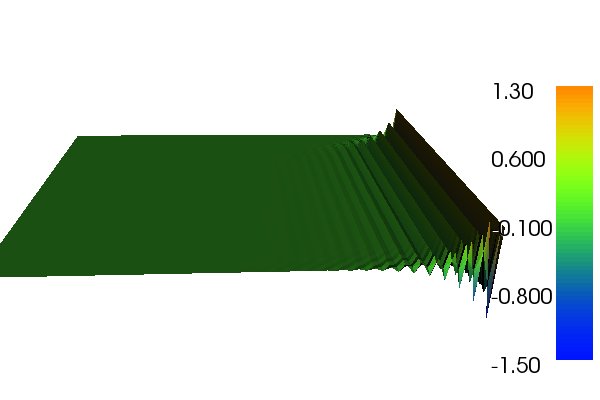
\includegraphics[width=\linewidth]{dolfin_plot_2.png}
  \caption{Plot of numerical solution u for $\mu=0.001$ and $h=64$, using normal Galerkin method. Notice oscillations close to $x=1$. }
  \label{Fig 3}
\end{figure}
\\
\\ 
The code is attached at the end together with the results. Could add, that to be able to define the exact solution for small $\mu$, I did the following approximation trick:
\begin{align*}
u(x,y)=\frac{1-e^{\frac{x}{\mu}}}{1-e^{\frac{1}{\mu}}} = \frac{e^{\frac{1}{\mu}}}{e^{\frac{1}{\mu}}}\frac{e^{-\frac{1}{\mu}}-e^{\frac{x-1}{\mu}}}{e^{-\frac{1}{\mu}}-1} = \frac{e^{-\frac{1}{\mu}}-e^{\frac{x-1}{\mu}}}{e^{-\frac{1}{\mu}}-1}  \approx e^{\frac{x-1}{\mu}}
\end{align*} 
This makes sense since $e^{-\frac{1}{\mu}} \approx 0 $ when $\mu$ is small.
\\
\\
As we see from the error results we get big errors in both norms when $\mu$ is small. To illustrate what happens I have plotted the numerical solution for $\mu=0.001$ and $h=64$. What we observe is oscillations close to $x=1$, where we now that the exact solution grows very fast.
\\
\\
c) Lets look at the convergence rate $\alpha$ and constant C, I get from $L^2$ and $H^1$ for different $\mu$.
\begin{center}
    \begin{tabular}{| l | l | l | l | l | l |}
    \hline
     & $\mu=1$ & $\mu=0.1$ & $\mu=0.01$ & $\mu=0.001$ & $\mu=0.0001$ \\ \hline
    $L^2$ $\alpha$ &  1.999763 & 1.975224 & 1.467166 & 1.299193& 1.802562\\ \hline
    $L^2$ C & 0.044866&  0.735446 &3.339322& 12.052507&301.737979\\ \hline
    $H^1$ $\alpha$ & 0.999856 &  0.978303 & 0.462191	& 0.184035& 0.698340\\ \hline
    $H^1$ C & 0.212219 &  4.229330 & 19.327090	& 44.796474&989.689148 \\ \hline
    \end{tabular}
\end{center}
As we see from these results, we get what we would expect for big $\mu$, but when we let $\mu$ get smaller, the convergence rate gets worse and the constant gets big. See that the convergence gets better again for the last $\mu$ value, but this is because error is so big that the convergence rate almost doesn't matter. The problem is that we get big oscillation near $x=1$. We see this by plotting, or that the $H1$ error gets big.
\\
\\
d) Want to implement the streamline upwind Petrov-Galerkin method. The notes describe how to do this when we use first order Lagrange elements. The only thing we have to add to our variational form is the term: 
\begin{align*}
\beta \int_{\Omega} (v\cdot \bigtriangledown u)(v\cdot \bigtriangledown w)dx = \beta\int_{\Omega} u_xw_xdx
\end{align*}
An important question is how to choose $\beta$. I choose to use $\beta \approx h$. This seemed to work. However, when I use a changing $\beta$, I can no longer use the sd norm to calculate the convergence rate of the method.
\\
\\
As above the code is attached below, and the error and convergence of the method is in the code as well. See that the $L^2$ error and $H^1$ error is much smaller for SUPG method then for the regular Galerkin method when $\mu$ is small. However, the convergence rate for $L^2$ is now a lot worse, and for $H^1$, the $H^1$ norm actually increases. To illustrate how much better SUPG is I have added a plot of the solution to the same problem I plotted above using SUPG. This looks a lot closer to the true solution, then what what we got earlier, i.e. no numerical artifacts. 
\begin{figure}
  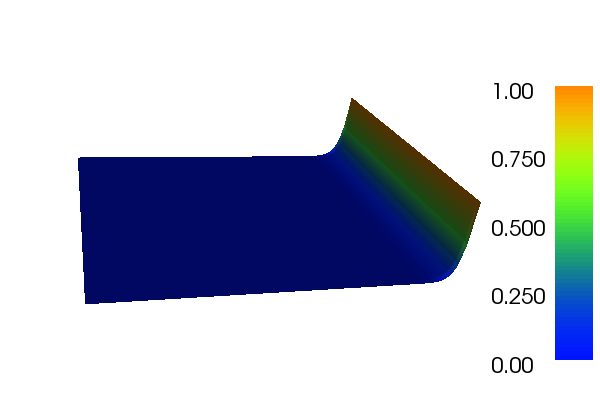
\includegraphics[width=\linewidth]{dolfin_plot_3.png}
  \caption{Plot of numerical solution u for $\mu=0.001$ and $h=64$ using the SUPG method. Notice that the graph is smooth, even at $x=1$. }
  \label{Fig 4}
\end{figure}
  
\lstdefinelanguage{Python}{
 keywords={typeof, null, catch, switch, in, int, str, float, self},
 keywordstyle=\color{ForestGreen}\bfseries,
 ndkeywords={boolean, throw, import},
 ndkeywords={return, class, if ,elif, endif, while, do, else, True, False , catch, def},
 ndkeywordstyle=\color{BrickRed}\bfseries,
 identifierstyle=\color{black},
 sensitive=false,
 comment=[l]{\#},
 morecomment=[s]{/*}{*/},
 commentstyle=\color{purple}\ttfamily,
 stringstyle=\color{red}\ttfamily,
}
\section*{Code for Exercise 1}
\lstinputlisting{Exersise1.py}
\section*{Code for Exercise 1}
\lstinputlisting{Exersise2.py}
\section*{Code for Exercise 1}
\lstinputlisting{SUPG_Exersise.py}
\end{document}
